%We conduct an empirical evaluation of the proposed algorithms.
%The goal is manifold.
We conducted extensive experiments to evaluate $(i)$\ the quality of our proposed algorithms, measured by the revenue achieved vis \`{a} vis the incentives paid to seed users,
% to achieve a certain level of revenue.
and $(ii)$\ the efficiency and scalability of the algorithms w.r.t. advertiser  budgets, which indirectly control the number of seeds required, and w.r.t. the number of advertisers, which effectively controls the size of the graph. %We measure both the running time and memory usage.
All experiments were run on a 64-bit OpenSuSE Linux server with Intel Xeon 2.90GHz CPU and 264GB memory.
As a preview, our largest configuration is \livej with 20 ads, which effectively yields a graph with $69M \times 20 \approx 1.4B$ edges; this is comparable with  \cite{tang14}, whose largest dataset has 1.5B edges.

\smallskip\noindent\textbf{Data.}
Our experiments were conducted on four real-world social networks, whose basic statistics are summarized in Table~\ref{table:dataset}.
We used \flix and \epi  for quality experiments and \dblp and \livej for scalability experiments.
\flix is from a social movie-rating website (\url{http://www.flixster.com/}),  which contains movie ratings by users along with timestamps.
\LL{We use the topic-aware influence probabilities and the item-specific topic distributions provided by Barbieri et al.~\cite{BarbieriBM12}, who learned the probabilities using MLE for the TIC model, with $L=10$ latent topics. We set the default number of advertisers $h=10$ and used five of the learned topic distributions from the provided \flix dataset, in such a way that every two ads are in pure competition, i.e., have the same topic distribution, with probability $0.91$ in one randomly selected latent topic, and $0.01$ in all others. This way, among $h=10$ ads, every two ads are in pure competition with each other while having a completely different topic distribution than the rest, representing a diverse marketplace of ads. \epi is a who-trusts-whom network taken from a consumer review website (\url{http://www.epinions.com/}). Likewise, we set $h=10$ and use the Weighted-Cascade model~\cite{kempe03}, where $p_{u,v}^i = 1/{|N^{in}(v)|}$ for all ads $i$. Notice that this corresponds to $L=1$ topic for \epi dataset, hence, all the ads are in pure competition.} % for the attention of  seed users.

\begin{table}[t!]
\vspace{-3mm}

\small
\centering
\caption{Statistics of network datasets.\label{table:dataset}}

\begin{tabular}{|c | c | c | c | c| }
\hline
& \flix & \epi  & \dblp & \livej  \\ \hline
\#nodes & 30K & 76K & 317K  & 4.8M \\ \hline
\#edges & 425K & 509K & 1.05M & 69M  \\ \hline
type & directed & directed & undirected & directed \\ \hline
\end{tabular}
%\vspace{-2mm}
\end{table}

\begin{table}[t!]
\small
\centering
\caption{Advertiser budgets and cost-per-engagement values.\label{table:cpe}}
	
\begin{tabular}{|c | c | c | c | c | c | c|}
		\hline
		 &  \multicolumn{3}{|c|}{ Budgets} & \multicolumn{3}{|c|} {CPEs} \\
 		 \hline
		 Dataset & mean & max  & min & mean & max & min  \\ \hline
		\flix & 10.1K  & 20K & 6K  & 1.5 & 2 & 1  \\ \hline
		\epi & 8.5K & 12K  & 6K  & 1.5 & 2 & 1 \\ \hline
	\end{tabular}
\vspace{1mm}
\end{table}

For scalability experiments, we used two large networks\footnote{\scriptsize Available at \url{http://snap.stanford.edu/}.} \dblp and \livej.
\dblp is a co-authorship graph (undirected) where nodes represent authors and there is an edge between two nodes if they have co-authored a paper indexed by DBLP. We direct all edges in both directions. \livej is an online blogging site where users can declare which other users are their friends.
In all datasets, advertiser budgets and CPEs were chosen in such a way that the total number of seeds required for all ads to meet their budgets is less  than $n$. This ensures that no ad is assigned an empty seed set.
For lack of space, instead of enumerating all CPEs and budgets, we give a statistical summary in Table~\ref{table:cpe}.
The same information for \dblp and \livej in provided later.

\spara{Seed incentive models.}
\LL{In order to understand how the algorithms perform w.r.t.\ different seed user incentive assignments, we used \AR{four} different methods that directly control the range between the minimum and maximum singleton payments:
%We assigned \emph{linear} seed user incentives that are proportional to the singleton influence spread of the nodes for each advertiser $i$, i.e., $c_i(u) = \alpha \cdot \sigma_i(\{u\})$, where $\alpha > 0$ is a fixed amount in dollar cents set by the host that directly controls how expensive the seed user incentives are, given the fixed budgets and CPEs of advertisers.
\squishlisttight
\item Linear incentives: proportional to the ad-specific singleton influence spread of the nodes, i.e., $c_i(u) = \alpha \cdot \sigma_i(\{u\}), \forall u \in V, i \in [h]$,
\item Constant incentives: the average of the ad-specific total linear seed user incentives, i.e., $c_i(u) = \alpha \cdot \dfrac{\sum_{v \in V}  \sigma_i(\{v\})}{n}, \forall u \in V, i \in [h]$,
\item Sublinear incentives: obtained by taking the logarithm of the ad-specific singleton influence spread of the nodes, i.e., $c_i(u) = \alpha \cdot \log(\sigma_i(\{u\})), \forall u \in V, i \in [h]$,
\item \AR{Superlinear incentives: obtained by using the squared ad-specific singleton influence spread of the nodes, i.e., $c_i(u) = \alpha \cdot \left(\sigma_i(\{u\})\right)^2, \forall u \in V, i \in [h]$},
\squishend
where $\alpha > 0$ denotes a fixed amount in dollar cents set by the host, which controls how expensive the seed user incentives are.
% cigdem: I remove this unit incentive, would confuse these reviewers..
%where $\alpha > 0$ denotes the ``unit incentive'', a fixed amount of dollar cents set by the host, which directly controls how expensive the seed user incentives are.
}


%%%%%%%%%%%%%%%%%% arxiv version of alpha-revenue plots (comment out for vldb submission)
%\eat{
\begin{figure}[t!]
\vspace{-4mm}
\begin{tabular}{ccc}
\vspace{-4mm}\includegraphics[width=.24\textwidth]{flix_alpha_totalRev_linear}&
	\hspace{-2mm}\includegraphics[width=.24\textwidth]{epi_alpha_totalRev_linear}&
\hspace{-4mm}\begin{sideways} $\;$ $\;\;$ $\;\;$ $\;\;$ $\;\;$ \textsf{\small Linear} \end{sideways} \\
\vspace{-4mm}\includegraphics[width=.24\textwidth]{flix_alpha_totalRev_uniform}&
	 \hspace{-2mm}\includegraphics[width=.24\textwidth]{epi_alpha_totalRev_uniform} &
\hspace{-4mm}\begin{sideways}  $\;$ $\;\;$ $\;\;$ $\;\;$ $\;\;$ \textsf{\small Constant} \end{sideways}\\
\vspace{-4mm}\includegraphics[width=.24\textwidth]{flix_alpha_totalRev_sublinear}&
	 \hspace{-2mm}\includegraphics[width=.24\textwidth]{epi_alpha_totalRev_sublinear} &
	  \hspace{-4mm}\begin{sideways} $\;$ $\;\;$ $\;\;$ $\;\;$ $\;\;$ \textsf{\small Sublinear} \end{sideways} \\
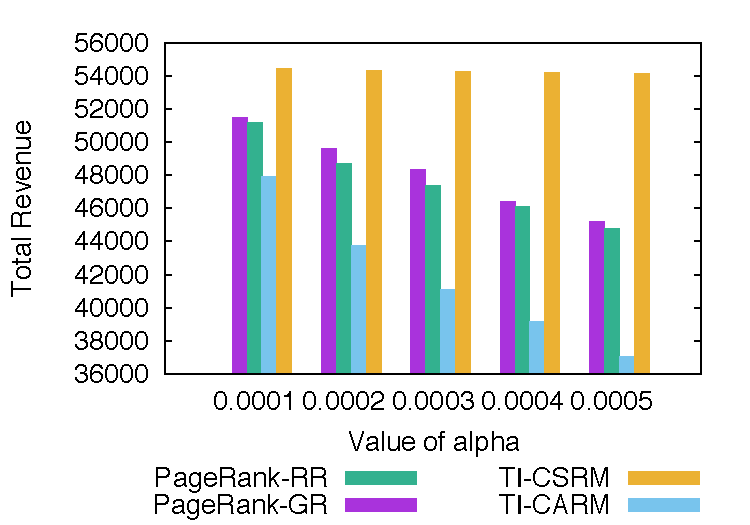
\includegraphics[width=.24\textwidth]{flix_alpha_totalRev_superlinear_legend}&
	 \hspace{-2mm}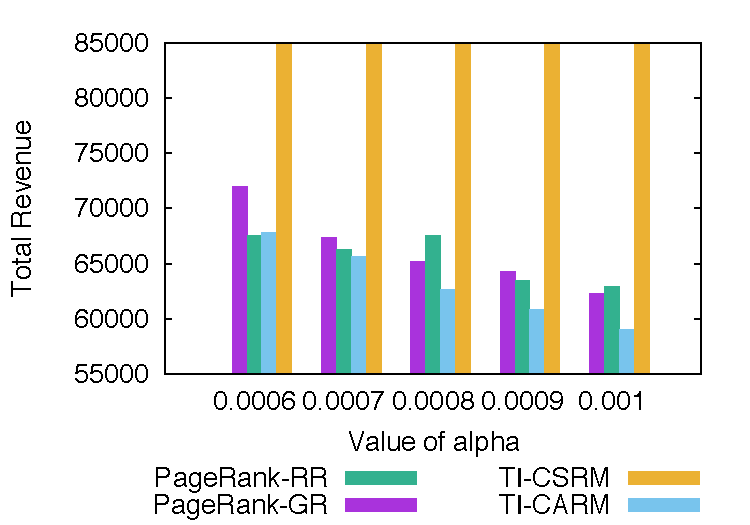
\includegraphics[width=.24\textwidth]{epi_alpha_totalRev_superlinear_legend} &
	  \hspace{-4mm}\begin{sideways} $\;$ $\;\;$ $\;\;$ $\;\;$ $\;\;$ \textsf{\small Superlinear} \end{sideways} \\ 	
\flix & \epi &
\end{tabular}
\caption{Total revenue as a function of $\alpha$, on \flix\ (left) and \epi\ (right), for linear, constant, sublinear, and superlinear incentive models.}
\label{fig:revenueAlphas}
\end{figure}
%}
%%%%%%%%%%%%%%%%%% vldb submission version of alpha-revenue plots (comment out for arxiv submission)
\eat{
\begin{figure}[t!]
\vspace{-4mm}
\begin{tabular}{ccc}
\vspace{-4mm}\includegraphics[width=.24\textwidth]{plots/alpha-nolegend/flix_alpha_totalRev_linear}&
	\hspace{-2mm}\includegraphics[width=.24\textwidth]{plots/alpha-nolegend/epi_alpha_totalRev_linear}&
\hspace{-4mm}\begin{sideways} $\;$ $\;\;$ $\;\;$ $\;\;$ $\;\;$ \textsf{\small Linear} \end{sideways} \\
\vspace{-4mm}\includegraphics[width=.24\textwidth]{plots/alpha-nolegend/flix_alpha_totalRev_uniform}&
	 \hspace{-2mm}\includegraphics[width=.24\textwidth]{plots/alpha-nolegend/epi_alpha_totalRev_uniform} &
\hspace{-4mm}\begin{sideways}  $\;$ $\;\;$ $\;\;$ $\;\;$ $\;\;$ \textsf{\small Constant} \end{sideways}\\
\includegraphics[width=.24\textwidth]{plots/alpha/flix_alpha_totalRev_sublinear}&
	 \hspace{-2mm}\includegraphics[width=.24\textwidth]{plots/alpha/epi_alpha_totalRev_sublinear} & \hspace{-4mm}\begin{sideways} $\;$ $\;\;$ $\;\;$ $\;\;$ $\;\;$ \textsf{\small Sublinear} \end{sideways} \\
\flix & \epi &
\end{tabular}
\caption{Total revenue as a function of $\alpha$, on \flix\ (left) and \epi\ (right), for linear (top), constant (middle), and sublinear (bottom) incentive models.}
\label{fig:revenueAlphas}
\end{figure}
}

On \flix and \epi we used Monte Carlo simulations (5K runs\footnote{\scriptsize We didn't observe any significant change in the influence spread estimation beyond 5K runs  for both datasets.}) to compute $\sigma_i(\{u\})$.  On \dblp and \livej, we use the out-degree of the nodes as a proxy to $\sigma_i(\{u\})$ due to the prohibitive computational cost of Monte Carlo simulations.
%\note[Laks]{Need to justify 5K runs. It sounds too small that I cannot recall seeing in any previous papers. Secondly, why couldn't we have used TIM/IMM to estimate the spread on \dblp and \livej instead of using out-degree? These questions need to be addressed.}
%\note[Cigdem]{For Epinions there was no difference between 5K and 10K runs. For INFLEX dataset that also uses the same Flixster TIC model, this was also the case so we always used 5K for INFLEX. Notice also that, we are not trying to estimate influence spread correctly here (also 10K is just a number which has no theoretical backing up). So I think we don't need to justify anything here but if you think it is necessary, we can maybe cite inflex to say that 5K versus 10K didn't matter, and add that for epinions this was also the case?
%For DBLP and LiveJ, it is not a good idea to use TIM since it wouldn't be giving us the singleton spread for all the nodes, and it is even a worse idea to use IMM since it just cares about top-k nodes. If we were to use TIM to assign seed costs, then it would have been a lot of correlation as we also use TIM to select the seeds, so we would be limiting the cost-sensitive algorithm's capability. }

%\input{old_tables.tex}

\smallskip\noindent\textbf{Algorithms.}
We compared \LL{four} algorithms in total. Wherever applicable, we set the parameter $\varepsilon$ to be $0.1$ for quality experiments on \flix and \epi, and $0.3$ for scalability experiments on \dblp and \livej, following the settings used in \cite{tang14}.

\squishlisttight
\item \fastcs (Algorithm~\ref{alg:fastCS}) that uses Algorithm~\ref{alg:rrBestCSNode} to find the best (cost-sensitive) candidate node for each advertiser (line~\ref{line:greedySelectBest}), and selects among those the (node, advertiser) pair that provides the maximum rate of marginal gain in revenue per marginal gain in advertiser's payment (line~\ref{line:greedyCriterCS}).
\item \fastca: Cost-agnostic version of Algorithm~\ref{alg:fastCS} that uses Algorithm~\ref{alg:rrBestCANode} to find the best (cost-agnostic) candidate node for each advertiser (replacing line~\ref{line:greedySelectBest}), and selects among those the (node, advertiser) pair with the maximum increase in the revenue of the host (replacing line~\ref{line:greedyCriterCS}).
\item \LL{PageRank-GR}: A baseline that selects a candidate node for each advertiser based on the ad-specific PageRank ordering of the nodes (replacing line~\ref{line:greedySelectBest}), and selects among those the (node, advertiser) pair that provides the maximum increase in the revenue of the host (replacing line~\ref{line:greedyCriterCS}). \textcolor{black}{Since the selection is made greedily, we refer to this algorithm as PageRank-GR.}
\item \LL{PageRank-RR: Another PageRank-based baseline that selects a candidate node for each advertiser based on the ad-specific PageRank ordering of the nodes (replacing line~\ref{line:greedySelectBest}), and uses a \textcolor{black}{Round-Robin (RR in short)} ordering of the advertisers for the assignment of their candidates into their seed sets.}
    %, while being mindful of the matroid constraint.}
\squishend

\smallskip\noindent\textbf{Revenue vs.\ $\alpha$.}
\LL{We first compare the total revenue achieved by the four algorithms for four different seed incentive models and with varying levels of $\alpha$ (Figure~\ref{fig:revenueAlphas}). Recall that by definition, a smaller %(resp.\ larger)
$\alpha$ value indicates lower %(resp.\ higher)
seed costs for all users. Across all different values of $\alpha$ and all seed incentive models, it can be seen that \fastcs consistently achieves the highest revenue, often by a large margin, which increases as $\alpha$ grows. For instance, on \epi, when $\alpha=0.5$, \fastcs achieved 15.3\%, {24.3\%}, 27.6\% more revenue than \fastca, {PageRank-RR, and PageRank-GR} respectively on the linear incentive model, while these values for superlinear incentive model respectively are 25.2\%, {25.8\%}, 18.1\%. Notice that for the constant incentive model, the advantage of being cost-sensitive is nullified, hence \fastca and \fastcs end up performing identically as expected.}
 \LL{Figure~\ref{fig:costAlphas} reports the cost-effectiveness of the algorithms. Across all different values of $\alpha$ and all incentive models, it can be seen that \fastcs consistently achieves the lowest total seed costs. This is as expected, since its seed allocation strategy takes into account revenue obtained per seed user cost.}

\AR{Notice that in three of the test cases, i.e., linear seed incentives on \flix and superlinear seed incentives on both datasets, \fastca has slightly worse performance than the two PageRank-based heuristics (e.g., about 4--7\% drop in revenue).} This can be explained by the fact that, while \fastca picks seeds of high spreading potential (i.e., highest marginal revenue) without considering costs, the two PageRank-based heuristics may instead select seeds of low quality (i.e., low marginal revenue), but also of very low cost. This might create a situation in which the PageRank-based heuristics may select many more seeds, but with a smaller total seed cost than \fastca, hence, allowing the budget to be spent more on engagements that translate to higher revenue, mimicking the cost-sensitive behavior. On the other hand \fastcs always spends the given budget judiciously by selecting seeds with the best rate of marginal revenue per cost. Thus, it is able to use the budget more intelligently, which explains its superiority in all test cases. This hypothesis is confirmed by our experiments. E.g., on \flix with linear seed incentives, we observed that the average values of marginal gain in revenue, seed user cost, and rate of marginal gain per cost obtained by PageRank-GR were respectively $2.67$, $0.44$, and $7.48$, while the corresponding numbers  for \fastca were $13.47$, $2.7$, and $4.89$, and those for \fastcs were $1.28$, $0.12$, and $9.95$ respectively. While the two PageRank-based heuristics could obtain higher revenue than \fastca on \flix with linear and superlinear incentives, and on \epi with superlinear incentives, they were greatly outperformed by \fastca, hence \fastcs, in the other incentive models, showing that such heuristics are not robust to different seed incentive models, and can only get ``lucky" to the extent they can mimic the cost-sensitive behavior.

%\LL{Notice that in one of the test cases, i.e., linear seed incentives on \flix, \fastca has slightly worse performance than the two PageRank-based heuristics (e.g., about 4--5\% drop in revenue). This can be explained by the fact that, while \fastca picks seeds of high spreading potential (i.e., highest marginal revenue) without considering costs, % and when it runs out of the budget, it stops.
%the two PageRank-based heuristics may instead select seeds of low quality (i.e., low marginal revenue), but also of very low cost.
%This might create a situation in which the PageRank-based heuristics may select many more seeds, but with a smaller total seed cost than \fastca.
%
%\LL{On the other hand \fastcs always selects seeds with the best
%rate of marginal revenue per cost. By doing so, it spends the given budget judiciously and is able to choose more seeds while using up the budget intelligently, which explains its superiority in all test cases. This hypothesis is confirmed by our experiments.
%%\note[Laks]{In the next sentence, two metrics are mentioned but three numbers! Also, it is not clear what the point being made is. Are metrics misalinged?}
%E.g., on \flix with linear seed incentives, we observed that the average marginal gain in revenue, seed user cost, and rate of marginal gain per cost obtained by PageRank-GR are respectively $2.67$, $0.44$, and $7.48$, while the corresponding numbers  for \fastca were $13.47$, $2.7$, and $4.89$, and those for \fastcs were $1.28$, $0.12$, and $9.95$ respectively. While the two PageRank-based heuristics could obtain higher revenue on \flix with linear seed incentives, they were greatly outperformed by \fastca, hence \fastcs, in the other incentive models, showing that such heuristics are not robust to different seed incentive models.}


%%%%%%%%%%%%%%%%%% arxiv version of alpha-cost plots (comment out for vldb submission)
%\eat{
\begin{figure}[t!]
\vspace{-4mm}
\begin{tabular}{ccc}
\vspace{-4mm}\includegraphics[width=.24\textwidth]{flix_alpha_totalCost_linear}&
	\hspace{-2mm}\includegraphics[width=.24\textwidth]{epi_alpha_totalCost_linear}&
\hspace{-4mm}\begin{sideways} $\;$ $\;\;$ $\;\;$ $\;\;$ $\;\;$ \textsf{\small Linear} \end{sideways} \\
\vspace{-4mm}\includegraphics[width=.24\textwidth]{flix_alpha_totalCost_uniform}&
	 \hspace{-2mm}\includegraphics[width=.24\textwidth]{epi_alpha_totalCost_uniform} &
\hspace{-4mm}\begin{sideways}  $\;$ $\;\;$ $\;\;$ $\;\;$ $\;\;$ \textsf{\small Constant} \end{sideways}\\
\vspace{-4mm}\includegraphics[width=.24\textwidth]{flix_alpha_totalCost_sublinear}&
	 \hspace{-2mm}\includegraphics[width=.24\textwidth]{epi_alpha_totalCost_sublinear} & \hspace{-4mm}\begin{sideways} $\;$ $\;\;$ $\;\;$ $\;\;$ $\;\;$ \textsf{\small Sublinear} \end{sideways} \\
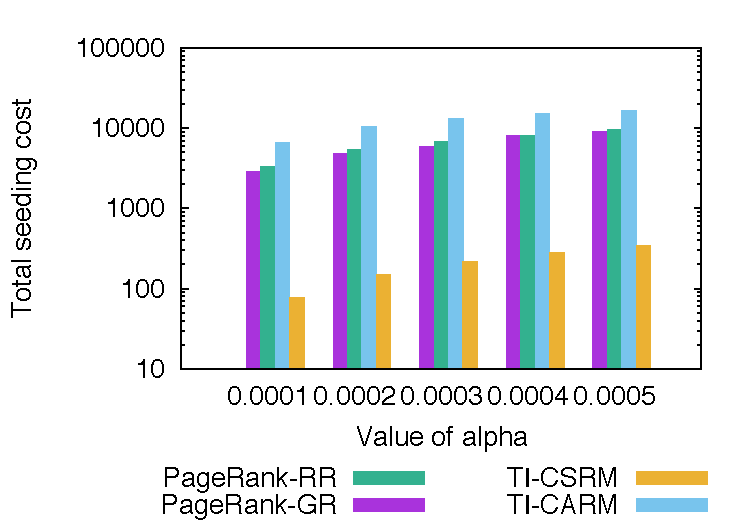
\includegraphics[width=.24\textwidth]{flix_alpha_totalCost_superlinear_legend}&
	 \hspace{-2mm}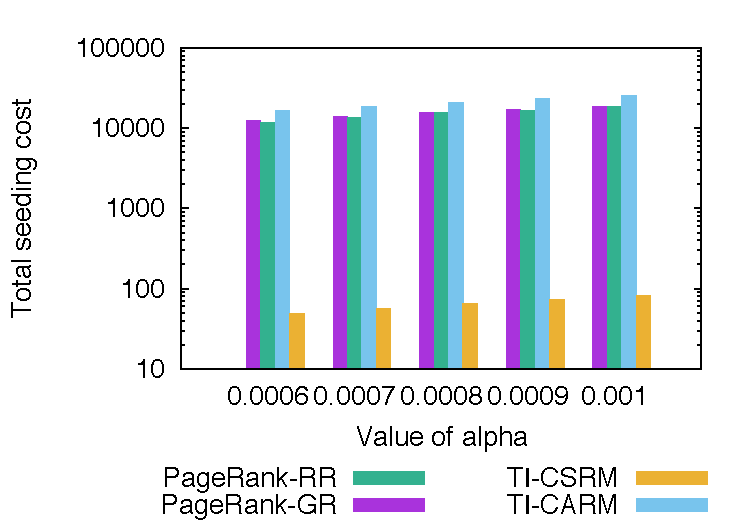
\includegraphics[width=.24\textwidth]{epi_alpha_totalCost_superlinear_legend} & \hspace{-4mm}\begin{sideways} $\;$ $\;\;$ $\;\;$ $\;\;$ $\;\;$ \textsf{\small Superlinear} \end{sideways} \\
\flix & \epi &
\end{tabular}
\caption{Total seeding cost as a function of $\alpha$, on \flix\ (left) and \epi\ (right), for linear, constant, sublinear, and superlinear cost models.}
\label{fig:costAlphas}
\end{figure}
%}
%%%%%%%%%%%%%%%%%% vldb submission version of alpha-cost plots (comment out for arxiv submission)
\eat{
\begin{figure}[t!]
\vspace{-4mm}
\begin{tabular}{ccc}
\vspace{-4mm}\includegraphics[width=.24\textwidth]{plots/alpha-nolegend/flix_alpha_totalCost_linear}&
	\hspace{-2mm}\includegraphics[width=.24\textwidth]{plots/alpha-nolegend/epi_alpha_totalCost_linear}&
\hspace{-4mm}\begin{sideways} $\;$ $\;\;$ $\;\;$ $\;\;$ $\;\;$ \textsf{\small Linear} \end{sideways} \\
\vspace{-4mm}\includegraphics[width=.24\textwidth]{plots/alpha-nolegend/flix_alpha_totalCost_uniform}&
	 \hspace{-2mm}\includegraphics[width=.24\textwidth]{plots/alpha-nolegend/epi_alpha_totalCost_uniform} &
\hspace{-4mm}\begin{sideways}  $\;$ $\;\;$ $\;\;$ $\;\;$ $\;\;$ \textsf{\small Constant} \end{sideways}\\
\includegraphics[width=.24\textwidth]{plots/alpha/flix_alpha_totalCost_sublinear}&
	 \hspace{-2mm}\includegraphics[width=.24\textwidth]{plots/alpha/epi_alpha_totalCost_sublinear} & \hspace{-4mm}\begin{sideways} $\;$ $\;\;$ $\;\;$ $\;\;$ $\;\;$ \textsf{\small Sublinear} \end{sideways} \\
\flix & \epi &
\end{tabular}
\caption{Total seeding cost as a function of $\alpha$, on \flix\ (left) and \epi\ (right), for linear (top), constant (middle), and sublinear (bottom) cost models.}
\label{fig:costAlphas}
\end{figure}
}

%\note[Cigdem]{Please check whether the paragraph below is clear and solid. I will also add a line to the discussion of Theorem~\ref{theo:cs-earm1} that our experiments verify theory.}
\CA{Finally, as shown in Figure~\ref{fig:revenueAlphas}, the extent to which  \fastcs outperforms \fastca on both datasets is higher with linear incentives than with sublinear incentives. For instance, on \flix, \fastcs achieved $45\%$ more revenue than \fastca in the linear model, while this improvement drops to $20\%$ in the sublinear model. To understand how the seeds' expensiveness levels affect this improvement, we checked the values of singleton payments and found that the maximum singleton payment ($\rho_{max}$) is $1347$ times more expensive than the minimum singleton payment ($\rho_{min}$) in the linear model, while it is $725$ times more expensive in the sublinear model that has lower improvement rate. This relation is expected as higher variety in the expensiveness levels of the seeds require to use the budget more cleverly, hence, with more cost-effective strategies. Notice that this finding is also in line with our discussion following the proof of Theorem~\ref{theo:cs-earm1}.}

It is also worth noting that, from Figure~\ref{fig:costAlphas}, \fastcs is two to three orders of magnitude more cost-efficient than the rest in the superlinear model, and this gap is larger than that attained in linear, constant, and sublinear scenarios.


%\textcolor{red}{It is also worth noting that, from Figure~\ref{fig:costAlphas}, \fastcs is two to three orders of magnitude more cost-efficient than the rest in the superlinear model, and this gap is larger than that attained in linear, constant, and sublinear scenarios.}

%\begin{figure}
%\centering
%\begin{tabular}{cc}
%\hspace{-4mm}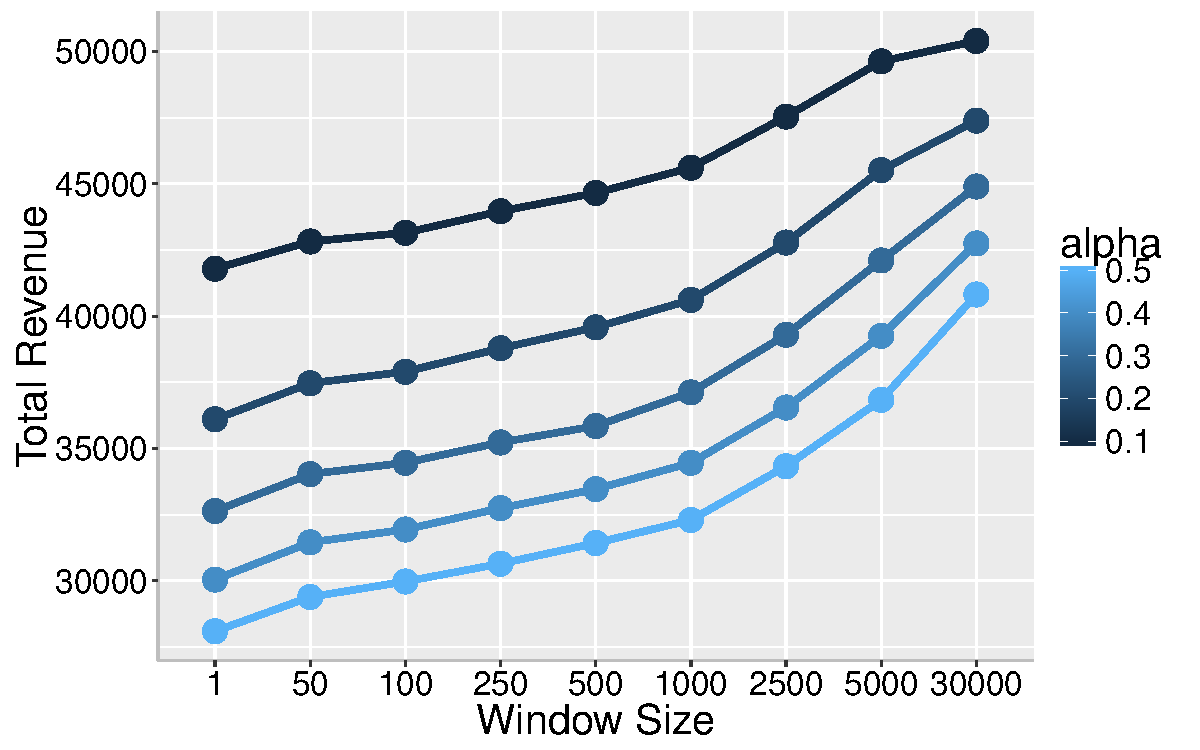
\includegraphics[width=.24\textwidth]{plots/window/flix-windows-Revenue_v2}&
%\hspace{-4mm}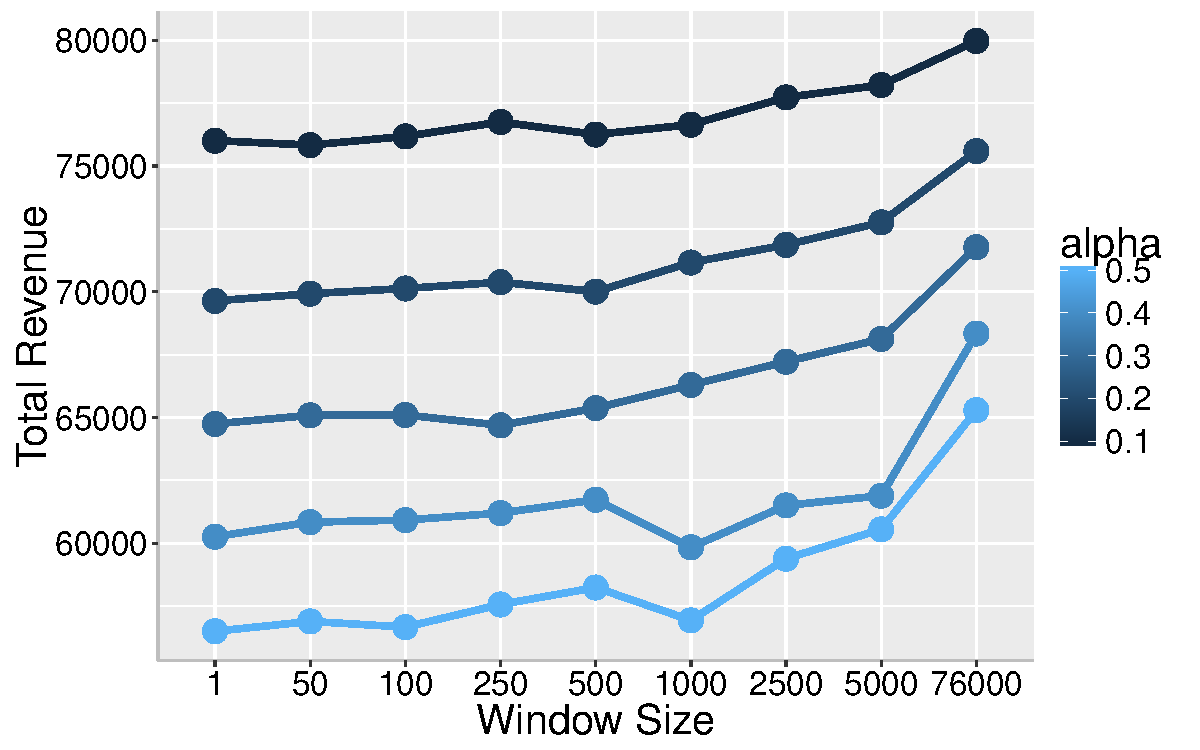
\includegraphics[width=.24\textwidth]{plots/window/epi-windows-Revenue_v2}\\
%\hspace{-4mm} (a) \flix  & \hspace{-4mm} (b) \epi
%\end{tabular}
%\caption{Revenue vs. window size with different $\alpha$}
%\label{fig:windowAlphas}
%\end{figure}




\smallskip\noindent\textbf{Revenue \& running time vs.\ window size.}
\textcolor{black}{Hereafter all presented results will be w.r.t.\ linear seed incentives, unless otherwise noted.}
As stated before in Section~\ref{sec:algorithms}, \fastcs needs to compute $\sigma_i(v | S^{t-1}_i)$, $\forall v : (v,i) \in \mathcal{E}^{t-1}$ while $u_i^{t}$ might even correspond to the node that has the \emph{minimum} marginal gain in influence spread for iteration $t$.
To have a closer look at how the revenue evolves when the seed selection criterion changes from cost-agnostic to cost-sensitive, we restrict  \fastcs to find the best cost-sensitive candidate nodes for each advertiser (line~\ref{line:greedySelectBest}) among only the $w$ nodes that have the highest marginal gain in revenue at each iteration. We refer to $w$ as the ``window size''.
Notice that \fastca corresponds to the case when $w=1$, i.e., in this case,  \fastcs inspects only the node with the maximum marginal gain in revenue.

We report the results of \fastcs with various window sizes in Fig.~\ref{fig:windowTradeoff}, which depicts the revenue vs. running time tradeoff.
Each figure corresponds to one dataset and one particular $\alpha$ value.
The $X$-axis is in log-scale.
As expected, the maximum revenue is achieved when \fastcs implements the full window $w = n$, \emph{i.e.}, when all the (feasible) nodes are inspected at each iteration for each advertiser.
The running time can go up quickly as the window size increases to $n$.
This is expected as the seed nodes selected do not necessarily provide high marginal gain in revenue, thus, \fastcs needs to use higher number of seed nodes, hence, much more RR-sets to achieve accuracy, compared to \fastca.

\begin{figure*}[t!]
\vspace{-4mm} %cide
\begin{tabular}{cccc}
    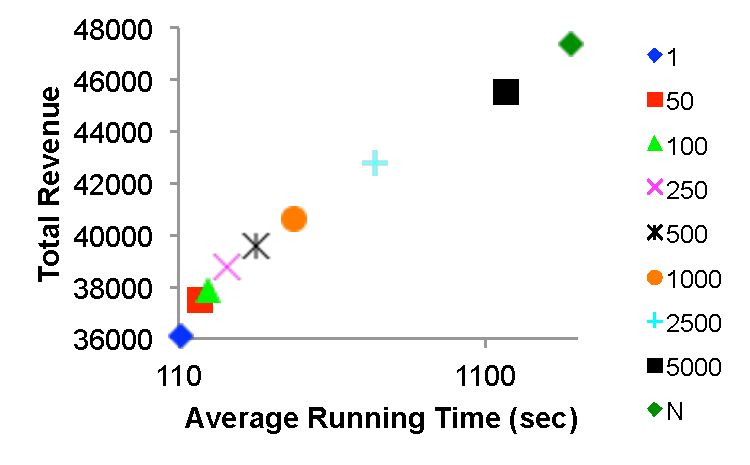
\includegraphics[width=.24\textwidth]{flix_rev_time_0_2}&
    \hspace{-2mm}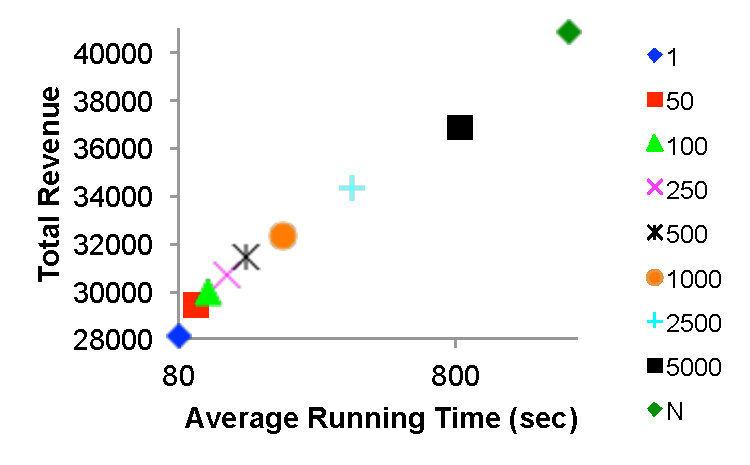
\includegraphics[width=.24\textwidth]{flix_rev_time_0_5}&
    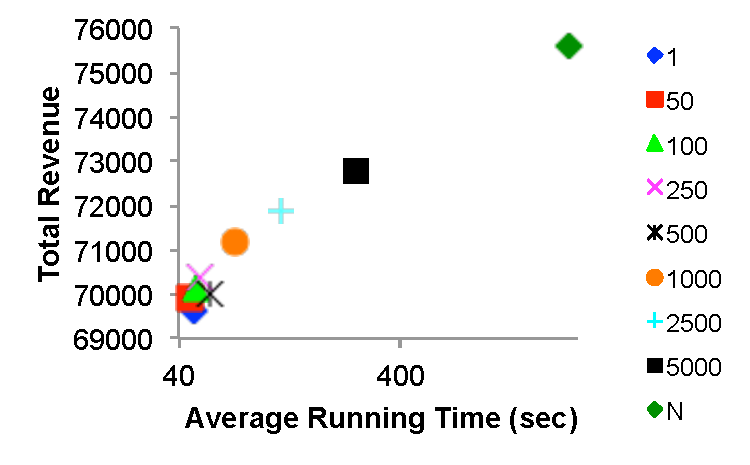
\includegraphics[width=.24\textwidth]{epi_rev_time_0_2}&
    \hspace{-2mm}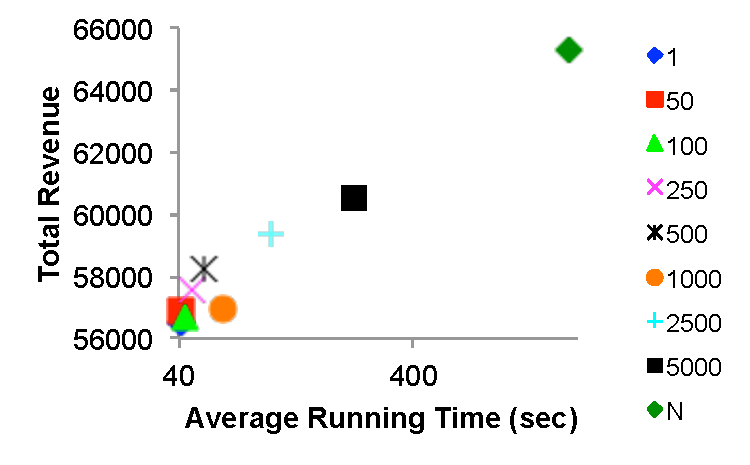
\includegraphics[width=.24\textwidth]{epi_rev_time_0_5}\\
	(a) \flix ($\alpha=0.2$)  & (b) \flix ($\alpha=0.5$) & (c)  \epi ($\alpha=0.2$) & (d) \epi ($\alpha=0.5$)   \\
\end{tabular}
\caption{Revenue vs running time tradeoff on \flix and \epi for two different value of $\alpha$.}
\label{fig:windowTradeoff}
\end{figure*}


\smallskip\noindent\textbf{Scalability.} We tested the scalability of \fastca and \fastcs on two larger graphs, \dblp and \livej. In all scalability experiments, we use a window size of $w = 5000$ nodes for \fastcs due to its good revenue vs running time trade-off. For simplicity, all CPEs were set to $1$.
The influence probability on each edge $(u,v)\in E$ was computed using the Weighted-Cascade model~\cite{kempe03}, where $p_{u,v}^i = 1/{|N^{in}(v)|}$ for all ads $i$.
We set $\alpha=0.2$ and $\varepsilon = 0.3$.
%We emphasize that our
This setting is well-suited for testing scalability as it simulates a fully competitive case: all advertisers compete for the same set of influential users (due to all ads having the same distribution over the topics), and hence it will ``stress-test'' the algorithms by prolonging the seed selection process.

Figure~\ref{fig:time}(a) and \ref{fig:time}(b) depict the running time of \fastca and \fastcs as the number of advertisers goes up from 1 to 20, while the budget is fixed (10K for \dblp and 100K for \livej).
As can be seen, the running time increases mostly in a linear manner, and \fastcs is only slightly slower than \fastca.
Figure~\ref{fig:time}(c) and \ref{fig:time}(d) depict the running time of \fastca and \fastcs as the budget increases, while the number of advertisers is fixed at $h=5$ .
We can also see that the increasing trend is mostly linear for \fastcs, while \fastca's time goes in a flatter fashion.
All in all, both algorithms exhibit decent scalability.

Table~\ref{table:mem} shows the memory usage of \fastca and \fastcs when $h$ increases. \fastcs in general needs to use higher memory than \fastca due to its requirement to generate more RR sets that ensures accuracy for using higher seed set size than \fastca.
On \dblp, \fastca and \fastcs respectively uses a total of $4676$ and $7276$ seed nodes for $h=20$.
On \livej \fastcs used typically between 20\% to 40\% more memory than \fastca: \fastca and \fastcs respectively uses a total of $4327$ and $6123$ seed nodes for $h=20$.

%\note[Wei]{\fastcs used more because of more RR sets? Why DBLP had almost identical numbers?}

\begin{table}
 \vspace{-4mm}
\centering
\small
 \caption{Memory usage (GB).\label{table:mem}}
 
  \begin{tabular}{|c|c|c|c|c|c|}
    \hline
    {\bf \dblp} & $h = 1$ & $5$ & $10$ & $15$ & $20$ \\ \hline
    \fastca &  1.6 & 7.5  & 14.9 & 22.4 &  29.8 \\ \hline
    \fastcs (5000) & 1.6 & 7.6 & 15.1 & 22.7 & 30.2 \\ \hline
    \hline
    {\bf \livej} & $h = 1$ & $5$ & $10$ & $15$ & $20$ \\ \hline
    \fastca & 2.5 & 12.1 & 25.3 & 39.4 &  54.4 \\ \hline
    \fastcs (5000) & 3.4 & 15.9 & 31.2 & 49.1 & 67.5  \\ \hline
  \end{tabular}
 \vspace{2mm}
\end{table}


\begin{figure*}
\begin{tabular}{cccc}
    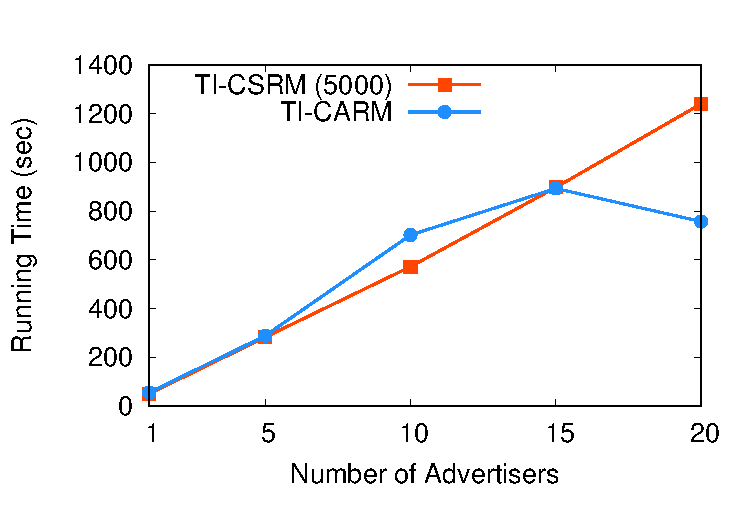
\includegraphics[width=.23\textwidth]{dblp_time_h}&
    \hspace{2mm}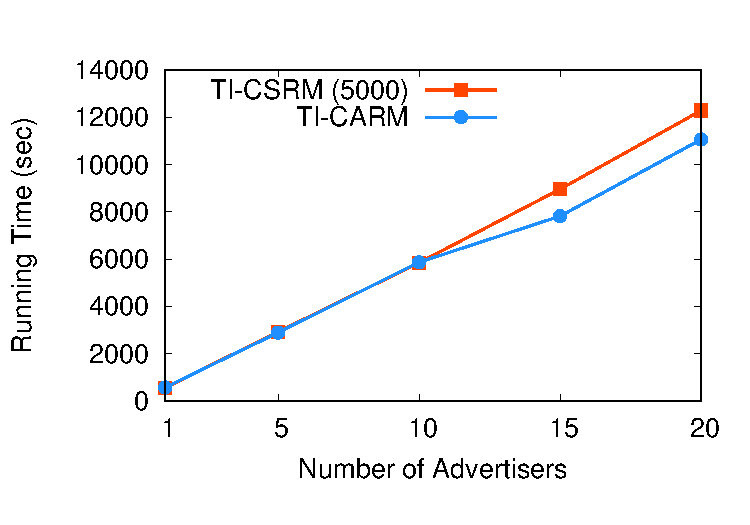
\includegraphics[width=.23\textwidth]{livej_time_h}&
    \hspace{2mm}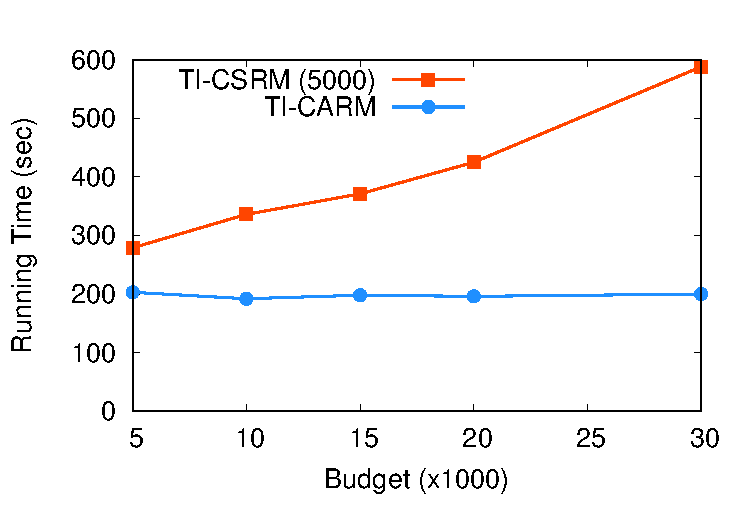
\includegraphics[width=.23\textwidth]{dblp_time_B}&
        \hspace{2mm}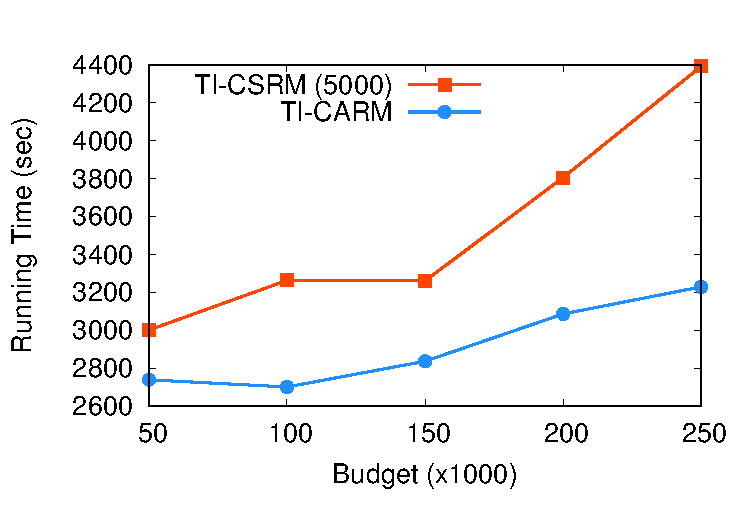
\includegraphics[width=.23\textwidth]{livej_time_B}\\
	(a) \dblp ($h$) & (b) \livej ($h$)   & (c) \dblp (budgets)  & (d) \livej (budgets)  \\
\end{tabular}
%\vspace{-2mm}
\caption{Running time of \fastca and \fastcs on \dblp and \livej}
\label{fig:time}
\end{figure*}
